\subsection{Theoretical Analysis} \label{subsec:intro}

\begin{tcolorbox}	
\begin{tabular}{p{2.75cm} p{0.2cm} p{10.5cm}}
\textbf{Contributors}  &:& Nelson Muga (2017-12-20 - )\\
                       &:& Diamantino Silva (2017-08-18 - ...)\\
                       &:& Armando Pinto (2017-08-15 - ...)\\
\textbf{Goal}          &:& Theoretical description of various optical detection schemes.\\
\end{tabular}
\end{tcolorbox}

The aim of this section is to calculate the signal to noise ratio at the input of the decision circuit for various detection schemes.
For each detection scheme a classical and a quantum description is going to be developed and a comparative analise is going to performed.

\subsubsection{Classical Description}

\begin{tcolorbox}	
\begin{tabular}{p{2.75cm} p{0.2cm} p{10.5cm}}
\textbf{Contributors}  &:& Nelson Muga (2017-12-20 - )\\
                       &:& Diamantino Silva (2017-08-18 - ...)\\
                       &:& Armando Pinto (2017-08-15 - ...)\\
\textbf{Goal}          &:& Develop a classical description of various optical detection schemes.\\
\end{tabular}
\end{tcolorbox}

{\bf \em Direct Detection}\\

One of the most simple detection methods is the direct detection of light with a single detector and the analise of the resulting photocurrent.

\begin{figure}[H]
	\label{fig:detection_direct}
	\centering
	
\includegraphics{./sdf/optical_detection/figures/detection-direct.pdf}
	\caption{Direct detection.}
\end{figure}

\noindent


Given an electric field generated by an ideal monochromatic single mode laser, it can be modulated in amplitude and phase by a signal $A(t)$ resulting in the function

\begin{equation}
    E_R(t)=\sqrt{2} |A(t)| cos\left(-\omega t + \theta\right) \,\,\,\, \sqrt{W}
\end{equation}
with $A(t)=|A(t)|e^{-i\theta(t)}$.

We will consider that the detector has a bandwidth $B$, greater that the signal $A(t)$, but much smaller than $2 \omega_0$. The calculation of power incident in the photodiode is given by the expected value of the square of the amplitude during a time interval $\Delta t = 2 \pi / \omega$\\

Measurable optical power, assuming that the detector bandwidth, $B$, is greater than the signal, $A(t)$, bandwidth but much small than $2 \omega_0$

\begin{align}
	P(t)	&= \overline{E_R^2(t)}\nonumber\\
			&= \overline{|A(t)|^2} + \overline{ |A(t)|^2 cos\left(-2 \omega t + 2\theta(t)\right)}\nonumber\\
         &= |A(t)|^2 \,\,\,\, W
\end{align}


\vspace{2em}
\noindent
To simplify calculations, the electric field can be expressed the complex notation
%
\begin{equation}
	E(t) = A(t) e^{-i \omega_0 t}
\end{equation}
%
%
The physically measurable quantities are obtained by taking the real part of the complex wave. Using this notation, the beam power, $P(t)$, is obtained by multiplying the electric field's conjugate by itself

\begin{align}
	P(t) &= E^{*}(t) E(t)\nonumber\\
         &= |A(t)|^2
\end{align}

\begin{equation}
	i(t) = \eta q \frac{P(t)}{\hbar \omega_0}
\end{equation}
in which $\eta$ is the photodiode's responsivity, q is the unit charge and $P(t)/\hbar \omega_0$ is the number of removed electrons.

The signal is ...
\begin{equation}
	E(t) = A(t) e^{-i \omega_0}
\end{equation}
Using the definition of electric power of a complex electric field representation, we will get
\begin{equation}
	P(t) = |A(t)|^2
	\label{eq:power}
\end{equation}
recovering the result of the real representation. The photocurrent can be rewriten as a function of the signal $A(t)$

\begin{equation}
	i(t) = \eta q \frac{|A(t)|^2}{\hbar \omega_0}
\end{equation}
which will use to express the second moment of the photocurrent as
\begin{equation}
	\langle i^2(t) \rangle = \eta^2 q^2 \frac{\langle |A(t)|^4 \rangle }{\hbar^2 \omega_0^2}
\end{equation}
Assuming a fase modulation, in which the amplitude is constant, the signal is simplified to
\begin{equation}
	A(t) = |A| e^{i \theta}
\end{equation}
Therefore, the current becomes constant
\begin{equation}
	i(t) = I_0 = \eta q \frac{A_s^2}{\hbar \omega_0}
\end{equation}
and it's second moment becomes simply
\begin{equation}
	\langle i^2(t) \rangle = I_0^2
\end{equation}

Shot noise in photodiodes\\

\begin{equation}
	\langle i_n^2(t) \rangle = 2 q B I_0
\end{equation}

The signal to noise ratio is obtained by the relation between the second moment of the sinal to the second moment of the noise

\begin{align}
	\frac{S}{N} &= \frac{\langle i^2(t) \rangle}{\langle i_n^2(t) \rangle} \nonumber\\
                &= \frac{I_0}{2 q B}\nonumber\\
                &= \eta \frac{ |A|^2}{\hbar \omega_0 B}
\end{align}

{\bf \em Homodyne Detection}\\

\begin{figure}[H]
	\centering
	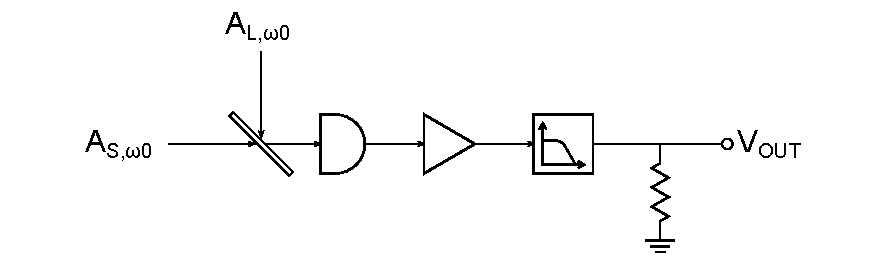
\includegraphics{./sdf/optical_detection/figures/detection-homodyne.pdf}
	\caption{Homodyne detection.}
\end{figure}
%%
The homodyne detection scheme uses an auxiliary local oscillator, which is combined in
a beamsplitter with the signal beam. After this step, it is similar to the direct detection. As we will see this has some implications in the phase detection???\\
\\
Given a splitter with intensity transmission $\epsilon$, the resulting field incident to the photodetector is
\cite{shapiro1985quantum} %p.241
%
\begin{equation}
	E(t) = \sqrt{\epsilon}E_S(t) + \sqrt{1-\epsilon}E_{LO}(t)
\end{equation}
%
in which $E_{LO} = e^{i \omega_0 t}$.
Given a local oscillator with a much larger power that the signal, then, the incident power in the photodiode is
%
\begin{align}
	P(t)	&= \eta \left[ (1-\epsilon) P_{LO}(t) + 2 \sqrt{\epsilon (1-\epsilon)} \textrm{Re} \left[ E_S(t) E^\ast_{LO}(t) \right] \right]\\
			&= \eta \left[ (1-\epsilon) P_{LO}(t) + 2 \sqrt{\epsilon (1-\epsilon)} |E_S(t)| |E_{LO}(t)| \cos{(\phi)} \right]\\
\end{align}

{\bf \em Balanced Homodyne Detection}\\
%
%

\begin{figure}[H]
	\centering
	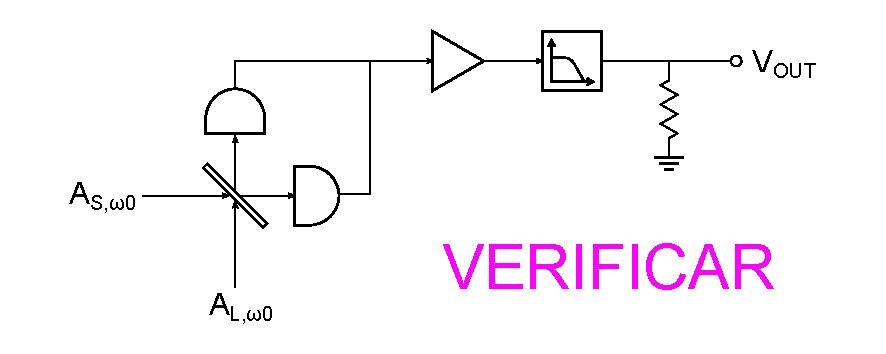
\includegraphics{./sdf/optical_detection/figures/detection-balanced-homodyne.pdf}
	\caption{Balanced homodyne detection.}
\end{figure}
%%
"In a balanced homodyne detector (BHD), the signal to be measured is mixed with a local oscillator (LO) at a beam splitter. The interference signals from the two output ports of the beam splitter are sent to two photodiodes followed by a subtraction operation, and then, amplification may be applied. The output of a BHD can be made to be proportional to either the amplitude quadrature or the phase quadrature of the input signal depending on the relative phase between the signal and the LO".
\\
\\
\\
{\bf \em IQ Homodyne Balanced Detection}\\

%%
\begin{figure}[H]
	\centering
	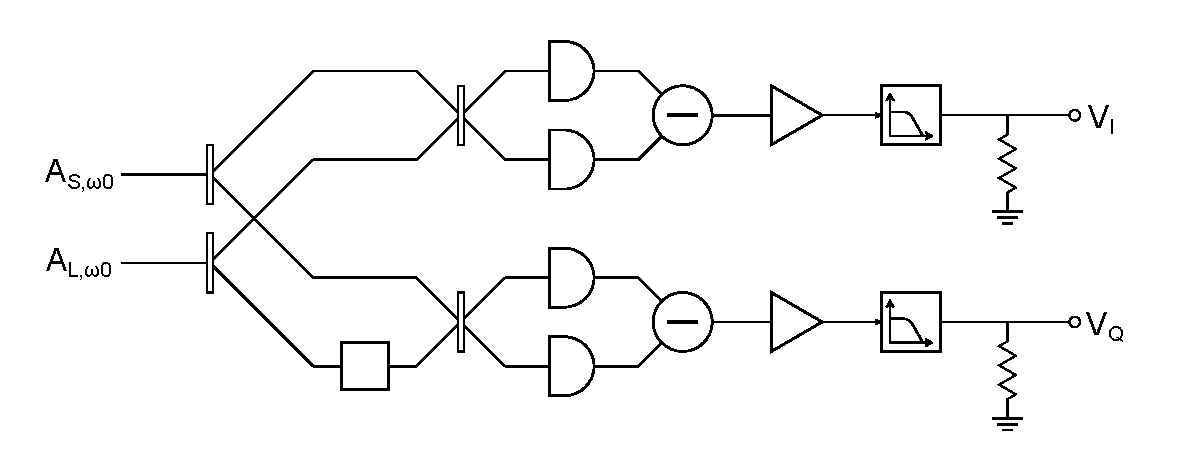
\includegraphics[width=15cm]{./sdf/optical_detection/figures/detection-IQ-balanced-homodyne.pdf}
	\caption{IQ balanced homodyne detection.}
\end{figure}
\noindent
{\bf \em Semiclassical model}\\
\\
{\bf \em Quantum model}\\


\paragraph{Heterodyne Detection}\ \\
%%
\begin{figure}[H]
	\centering
	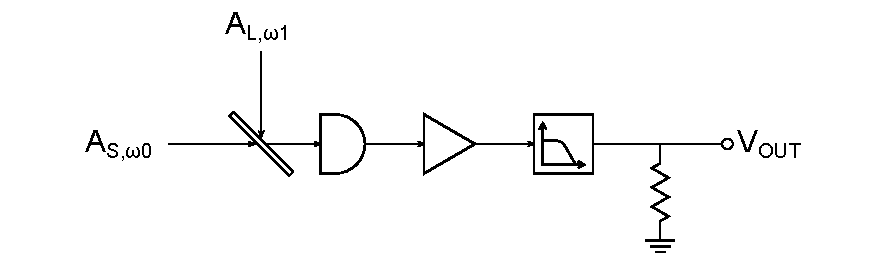
\includegraphics{./sdf/optical_detection/figures/detection-heterodyne.pdf}
	\caption{Heterodyne detection.}
\end{figure}

% inventado
In contrast with the homodyne detection, in which the frequency of the signal carrier is equal to the frequency of the local oscillator, in the heterodyne detection, these frequencies are different.\\
Because of this, the inference will result in a new signal with an intermediate frequency at...\\
% PROCURAR REFERENCIAS
\\



\paragraph{Balanced Heterodyne Detection}\ \\
%%
\begin{figure}[H]
	\centering
	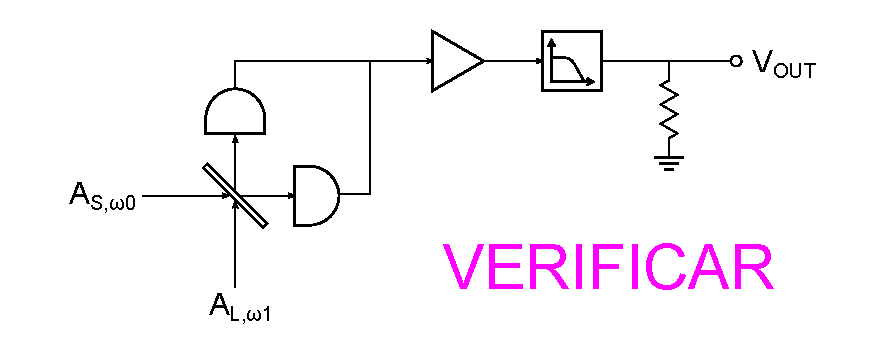
\includegraphics{./sdf/optical_detection/figures/detection-balanced-heterodyne.pdf}
	\caption{Balanced heterodyne detection.}
\end{figure}
%
\noindent
{\bf \em Semiclassical model}\\
\\
{\bf \em Quantum model}\\


\paragraph{IQ Heterodyne Balanced Detection}\ \\
%
\begin{figure}[H]
	\centering
	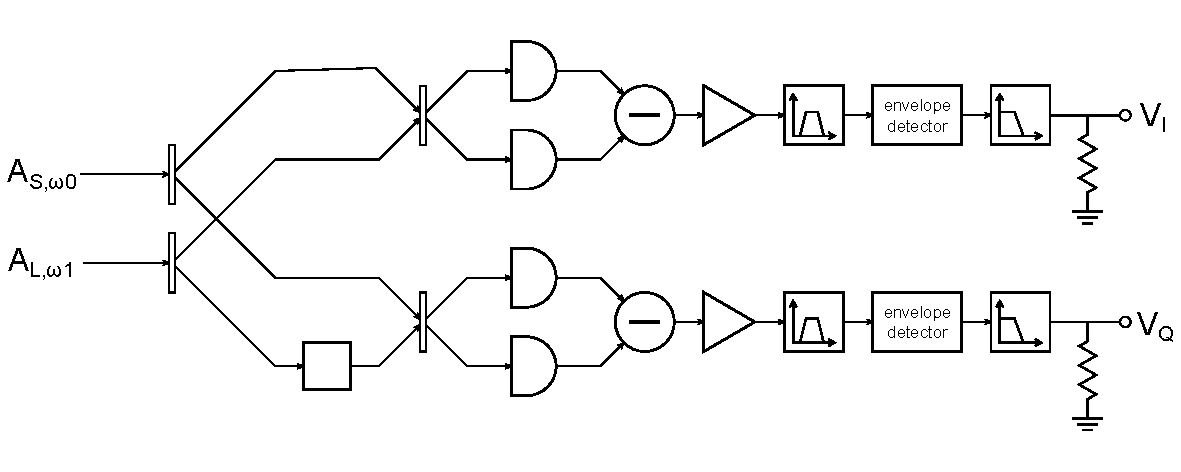
\includegraphics[width=15cm]{./sdf/optical_detection/figures/detection-IQ-balanced-heterodyne.pdf}
	\caption{IQ balanced heterodyne detection.}
\end{figure}
%
\noindent
\subsubsection{Thermal noise}
Thermal noise is generated by electrons in response to temperature. It's contribution to the resulting current can be described by the following equation
\cite{fox2006}
%\footnote{Mark Fox, p. 96}
%
\begin{equation}
\braket{(\Delta i_T)^2} = 4 K_B T_0 B/R_L
\end{equation}
%
in which $K_B$ it's Boltzmann's constant, $T_0$ is the absolute temperature, $B$ is the bandwidth and $R_L$ is the receiver load impedance. The $B$ value is imposed by default or chosen when the measurements are made, but the $R_L$ value is dependent in the internal setup of the various components of the detection system. Nevertheless, for simulation purposes, we can just introduce an experimental value.\\
\vspace{1cm}
%
%


\subsubsection{Quantum Description}

\begin{tcolorbox}	
\begin{tabular}{p{2.75cm} p{0.2cm} p{10.5cm}}
\textbf{Contributors}  &:& Diamantino Silva (2017-08-18 - ...)\\
                       &:& Armando Pinto (2017-08-15 - ...)\\
\textbf{Goal}          &:& Develop a quantum description of various optical detection schemes, and compare with the classical description.\\
\end{tabular}
\end{tcolorbox}

We start by defining number states $\ket{n}$ (or Fock states), which correspond to states with perfectly fixed number of photons
%\footnote{Loundon, p.184}
\cite{loudon2000}.
Associated to those states are two operators, the creation $\hat{a}^\dagger$ and annihilation $\hat{a}$ operators, which in a simple way, remove or add one photon from a given number state
%\footnote{Mark Fox, p.155}
\cite{fox2006}.
Their action is defined as
%
\begin{center}
	\hspace{-4mm}
	\begin{minipage}{44mm}
		\noindent
		\begin{equation}
			\hat{a} \ket{n} = \sqrt{n} \ket{n-1}
		\end{equation}
	\end{minipage}
	$,\quad$
	\begin{minipage}{52mm}
		\noindent
		\begin{equation}
			\hat{a}^\dagger \ket{n} = \sqrt{n+1} \ket{n+1}
		\end{equation}
	\end{minipage}
	$,\quad$
	\begin{minipage}{35mm}
		\noindent
		\begin{equation}
			\hat{n} \ket{n} = n \ket{n}
		\end{equation}
	\end{minipage}
\end{center}
%
in which $\hat{n} = \hat{a}^\dagger\hat{a}$ is the number operator. Therefore, number states are eigenvectors of the number operator.\\
\\
Coherent states have properties that closely resemble classical electromagnetic waves, and are generated by single-mode lasers well above the threshold.
\cite{loudon2000}
%\footnote{Loudon, p.190}
We can defined them, using number states in the following manner
\begin{equation}
\ket{\alpha} = e^{-\frac{|\alpha|^2}{2}} \sum_{n=0}^\infty \frac{\alpha^n}{\sqrt{n!}} \ket{n}
\end{equation}
in which the complex number $\alpha$ is the sole parameter that characterizes it.
%\footnote{Loudon, p.184}
%\footnote{Loudon, p.186}
In fact, if we calculate the expected number of photons with $\bra{\alpha} \hat{n} \ket{\alpha}$ we will obtain $|\alpha|^2$. The coherent state is an eigenstate of the annihilation operator, $\hat{a}\ket{\alpha} = \alpha \ket{\alpha}$.\\
\\
%
%
Using the creation and annihilation operators, we can define two quadrature operators
\cite{loudon2000}
%\footnote{Loudon, p.138, (4.3.36)}
%
\begin{center}
	\begin{minipage}{41mm}
		\noindent
		\begin{equation}
			\hat{X} = \frac{1}{2} \left( \hat{a}^\dagger + \hat{a} \right)
		\end{equation}
	\end{minipage}
	$,\quad$
	\begin{minipage}{40mm}
		\noindent
		\begin{equation}
			\hat{Y} = \frac{i}{2} \left( \hat{a}^\dagger - \hat{a} \right)
		\end{equation}
	\end{minipage}
\end{center}
%
The expected value of these two operators, using a coherent state $\ket{\alpha}$ are
%
\begin{center}
	\begin{minipage}{37mm}
		\noindent
		\begin{equation}
			\braket{\hat{X}} = \textrm{Re}(\alpha)
		\end{equation}
	\end{minipage}
	$,\quad$
	\begin{minipage}{37mm}
		\noindent
		\begin{equation}
			\braket{\hat{Y}} = \textrm{Im}(\alpha)
		\end{equation}
	\end{minipage}
\end{center}
%
We see that the expected value of these operators give us the real and imaginary part of $\alpha$. Now, we can obtain the uncertainty of these operators, using:
%
\begin{equation}
\textrm{Var}(\hat{X}) = \braket{\hat{X}^2} - \braket{\hat{X}}^2
\end{equation}
%
For each of these quadrature operators the variance will be
%
\begin{equation}
\textrm{Var}(\hat{X}) = \textrm{Var}(\hat{Y}) = \frac{1}{4}
\end{equation}
%
This result show us that for both quadratures, the variance of measurement is the same and independent of the value of $\alpha$.
%
%
%
\subsubsection{Homodyne detection}

The measurent of a quadrature of an input signal (S) is made by using the balanced homodyne detection technique, which measures the phase difference between the input signal and a local oscillator (LO). The measurement of quadrature are made relative to a reference phase of the LO, such that if the measurement is made in-phase with this reference, the value will be proportional to the $\hat{X}$ quadrature of the signal. If the phase of the LO is has an offset of $\pi/2$ relative to the reference, the output will be proportional to the $\hat{Y}$ quadrature of the signal.\\
\\
Experimentally, the balanced homodyne detection requires a local oscillator with the same frequency as the input signal, but with a much larger amplitude. These two signals are combined using a 50:50 beam splitter, from were two beams emerge, which are then converted to currents using photodides. Finally, the two currents are subtracted, resulting in an output current proportional to a quadrature of the input signal
\cite{fox2006}.\\
%\footnote{Mark Fox, p. 140}
%
%The balanced homododyne technique is used to measure the phase of the input signal (S), relative to the phase of a local oscillator (LO), which has the same frequency as the input signal, but a much larger amplitude. The technique consists in combining the input signal and the local oscillator, using a 50:50 beam splitter, from whom two beams emerge, which are then converted to currents using photodides. Finally, the two currents are subtracted, resulting in an output current.\\
A phase of the local oscillator can be defined as the reference phase. A phase offset equal to $0$ or $\pi/2$ will give an output proportional to the signal's in-phase component or to the quadrature component, respectively. Therefore, the $\hat{X}$ operator will correspond to the in-phase component and $\hat{Y}$ operator correspond to quadrature component
%\cite{fox2006}.
%\footnote{Mark Fox, p. 140}
\\
%
\begin{figure}[H]
	\label{fig:scheme_homodyne}
	\centering
	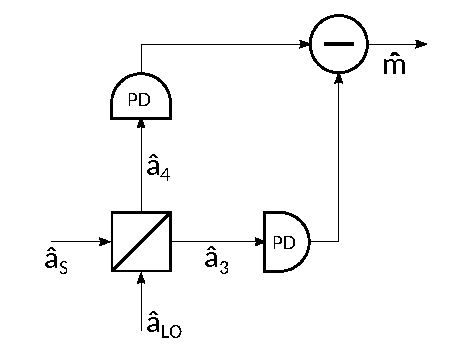
\includegraphics{./sdf/optical_detection/figures/scheme_homodyne.pdf}
	\caption{Balanced homodyne detection.}
\end{figure}
%
In the lab and in our simulations, a more complex system is used, the double balanced homodyne detection, which allows the simultaneous measurement of the $\hat{X}$ and $\hat{Y}$ components. The signal is divided in two beam with half the power of the original. One of the beams is used in a balanced homodyne detection with a local oscillator. The other beam is used in another balanced homodyne detection, but using a local oscillator with a phase difference $\pi/2$ relative to the first one.
%
\begin{figure}[H]
	\label{fig:scheme_homodyne}
	\centering
	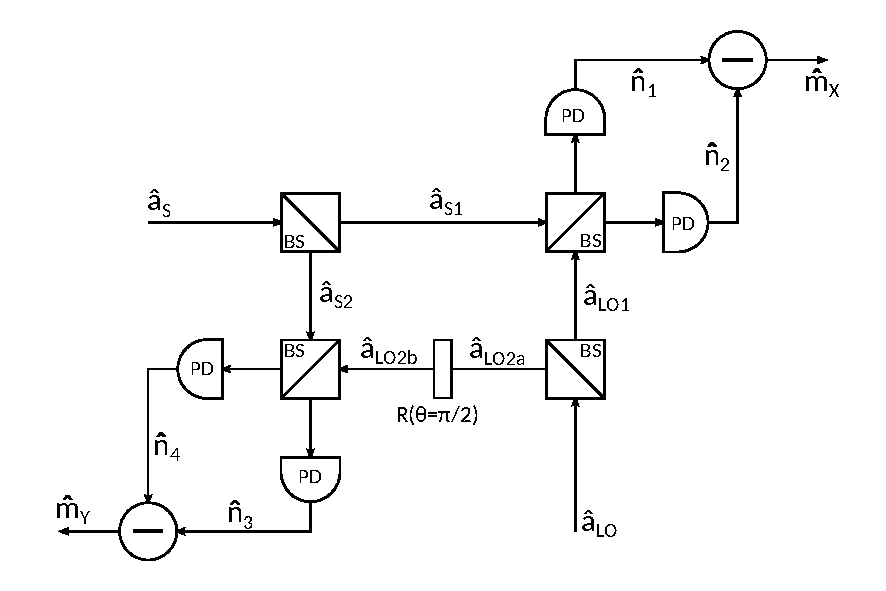
\includegraphics{./sdf/optical_detection/figures/scheme_double_homodyne.pdf}
	\caption{Balanced double homodyne detection.}
\end{figure}
%
%
%
\subsubsection{Noise sources in homodyne detection}
The detection of light using photodiodes is subjected to various sources of noise. One of these sources is the electrical field itself. The interaction of the signal with the vaccuum field adds quantum noise to the detection.
Another source of noise comes from the detection system, such as photodiodes and other electrical circuits, originating various kinds of noise, such as thermal noise, dark noise and amplifier noise
%\footnote{Hans, p.185}
\cite{hans2004}.
In the following sections, we will focus on two noise sources, quantum noise and thermal noise.
%
%
%
\subsubsection{Quantum Noise}
In order to grasp this effect, the quantum mechanical description of balanced homodyne detection will be used, employing quantum operators to describe the effect of each component in the system (fig. \ref{fig:scheme_homodyne}). We start with the operators $\hat{a}_S$ and $\hat{a}_{LO}$ corresponding to the annihilation operator for the signal and local oscillator, which are the inputs in a beam divisor. The outputs will be $\hat{a}_3$ and $\hat{a}_4$.
Using a balanced beam splitter, we can write the output as
%
\begin{center}
	\begin{minipage}{48mm}
		\noindent
		\begin{equation}
			\hat{a}_3 = \frac{1}{\sqrt{2}} \left( \hat{a}_S + \hat{a}_{LO} \right)
		\end{equation}
	\end{minipage}
	$,\quad$
	\begin{minipage}{48mm}
		\noindent
		\begin{equation}
			\hat{a}_4 = \frac{1}{\sqrt{2}} \left( \hat{a}_S - \hat{a}_{LO} \right)
		\end{equation}
	\end{minipage}
\end{center}
%
The final output of a homodyne measurement will be proportional to the difference between the photocurrents in arm $3$ and $4$. Then
%
\begin{equation}
I_{34} = I_3 - I_4 \sim \braket{\hat{n}_3 - \hat{n}_4}
\end{equation}
%
We can define an operator that describes the difference of number of photons in arm 3 and arm 4:
%
\begin{equation}
\hat{m} = \hat{a}^\dagger_3\hat{a}_3 - \hat{a}^\dagger_4\hat{a}_4
\end{equation}
%
If we assume that the local oscillator produces the the coherent state $\ket{\beta}$, then the expected value of this measurement will be
%
\begin{center}
	\begin{minipage}{58mm}
		\noindent
		\begin{equation}
			\braket{m} = 2|\alpha||\beta|\cos({\theta_\alpha - \theta_\beta})
		\end{equation}
	\end{minipage}
	$,\quad$
	\begin{minipage}{46mm}
		\noindent
		\begin{equation}
			\textrm{Var}(m) = |\alpha|^2 + |\beta|^2
		\end{equation}
	\end{minipage}
\end{center}
%
The local oscillator normally has a greater power than the signal
%VER REFERENCIAS
, then $|\alpha| \ll |\beta|$. If we use as unit, $2|\beta|$, then these two quantities can be simplified to
%
\begin{center}
	\begin{minipage}{52mm}
		\noindent
		\begin{equation}
			\label{eq:var_m}
			\braket{m} = |\alpha|\cos({\theta_\alpha - \theta_\beta})
		\end{equation}
	\end{minipage}
	$,\quad$
	\begin{minipage}{34mm}
		\noindent
		\begin{equation}
			\textrm{Var}(m) \approx \frac{1}{4}
		\end{equation}
	\end{minipage}
\end{center}
%
\cite{hans2004}
%\footnote{Referencia indirecta: Livro: Hans, p.207}
\\
Has we have seen previously, in order to measure two quadratures simultaneously, we can use double balanced homodyne detection. For each quadrature, the input signal now has half the power, so $|\alpha| \rightarrow |\alpha/\sqrt{2}|$.  If we use a local oscillator that produces states $\ket{\beta}$, then we can divide it in two beams in state $\ket{\beta/\sqrt{2}}$ and $\ket{i\beta/\sqrt{2}}$ which will be used in each homodyne detection. In this setting, the expected values for each quadrature, $X$ and $Y$, (in normalized values of $\sqrt{2}|\beta|$) are
%
\begin{center}
	\begin{minipage}{58mm}
		\noindent
		\begin{equation}
			\braket{m_X} = \left|\frac{\alpha}{\sqrt{2}}\right| \cos({\theta_\alpha - \theta_\beta})
		\end{equation}
	\end{minipage}
	$,\quad$
	\begin{minipage}{37mm}
		\noindent
		\begin{equation}
			\textrm{Var}(m_X) \approx \frac{1}{4}
		\end{equation}
	\end{minipage}
\end{center}
%
%
\begin{center}
	\begin{minipage}{58mm}
		\noindent
		\begin{equation}
			\braket{m_Y} =  \left|\frac{\alpha}{\sqrt{2}}\right| \sin({\theta_\alpha - \theta_\beta})
		\end{equation}
	\end{minipage}
	$,\quad$
	\begin{minipage}{37mm}
		\noindent
		\begin{equation}
			\textrm{Var}(m_Y) \approx \frac{1}{4}
		\end{equation}
	\end{minipage}
\end{center}
%
Therefore the measurement of each quadrature will have half the amplitude, but the same variance.
%
%
%